\section{Data Driven Security}%
\label{sec:data_driven_security}

Durch Datenanalyse kann das Risiko eines einzelnen Pakets ermittelt werden.
Mit der Zeit wurden viele Modelle und Ansätze entwickelt um Außenseiter zu erkennen.

\subsection{Problem}%
\label{sub:problem}

Die \emph{guten} Daten sollen von den \emph{schlechten} Daten unterschieden werden.
Weiterhin sollen die am besten passenden Charakteristika und Prozeduren gefunden werden,
die unser Problem lösen und uns helfen das System besser zu verstehen.

\begin{figure}[h]
  \centering
  \begin{subfigure}[c]{0.45\textwidth}
    \centering
    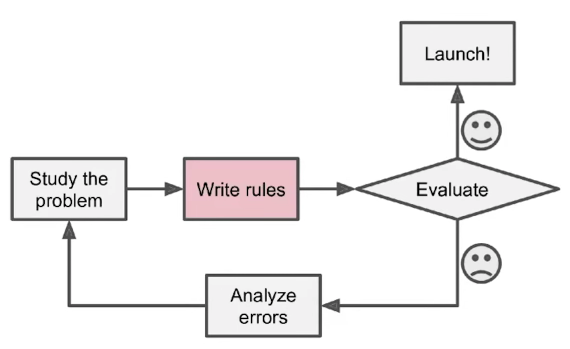
\includegraphics[width=0.95\linewidth]{bilder/without_ml.png}
    \subcaption{ohne Machine Learning}
    \label{fig:without_ml}
  \end{subfigure}
  \begin{subfigure}[c]{0.45\textwidth}
    \centering
    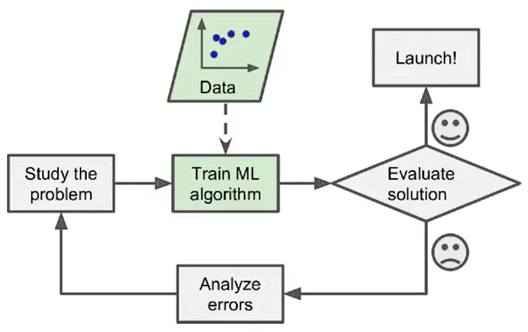
\includegraphics[width=0.95\linewidth]{bilder/with_ml.png}
    \subcaption{mit Machine Learning}
    \label{fig:with_ml}
  \end{subfigure}
  \caption{Problemlösen}
\end{figure}

Um das Problem besser zu verstehen, kann auch ML genutzt werden:
\begin{figure}[h]
  \centering
  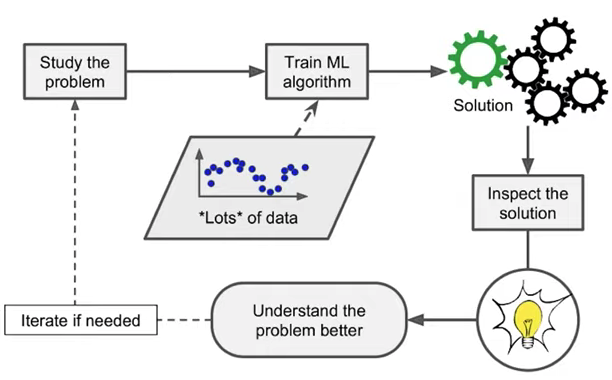
\includegraphics[width=0.6\linewidth]{bilder/human_learning_with_ml.png}
  \caption{Menschliches Lernen mit Hilfe von ML}
  \label{fig:human_learning_with_ml}
\end{figure}

\subsection{Lernen von Daten}%
\label{sub:lernen_von_daten}

\begin{description}
  \item[Domänenexpertise] um unser Fachwissen zu vergrößern
  \item[Datenmanagement] die Daten vorbereiten, speichern und warten
  \item[Programmierung] um Daten mit Analysen zu verbinden
  \item[Statistiken] um von den Daten zu lernen
  \item[Visualisierung] um die Ergebnisse effektiv zu kommunizieren
\end{description}

\subsection{Klassifizierung von ML Systemen}%
\label{sub:klassifizierung_von_ml_systemen}

Es gibt verschiedene Kategorien:
\begin{itemize}
  \item ob sie unter menschlicher Aufsicht trainiert werden
    (supervised, unsupervised, semi-supervised, reinforcement learning)
  \item ob sie inkrementell on the fly lernen können (online vs. batch learning)
  \item ob sie einfach nur neue Daten mit bekannten Daten vergleichen
    oder Muster erkennen und daraus wie Wissenschaftler ein Vorhersagemodell erzeugen
    (instance based vs. model-based learning)
\end{itemize}

\subsubsection{Supervised Learning}%
\label{ssub:supervised_learning}

Hier gibt’s Trainingsdaten mit Labels, mit der der Algorithmus gefüttert wird.
Dann wird der Algorithmus mit Testdaten getestet, bei denen die Labels fehlen.
Beispiele: Spamerkennung, Vorhersage von Werten mittels Regression.

Ein Parameter mit Wert der Daten wird \emph{Attribut} oder \emph{Feature} genannt.
Beispiel: ein gesetztes Flag in einem TCP-Paket.

\paragraph{Klassifikation}%
\label{par:klassifikation}

Heißt die Aufteilung in Klassen.
Trainiert wird mit Daten, deren Klasse bekannt ist und ein Label hat.

\paragraph{Regression}%
\label{par:regression}

Die Aufgabe hierbei ist einen numerischen Zielwert vorherzusagen, bspw. die Gefahr eines
IP-Pakets, anhand einer Menge von Features.
Das nennt man \emph{Prädiktor}.

\paragraph{Beste bekannte Algorithmen}%
\label{par:beste_bekannte_algorithmen}

\begin{itemize}
  \item $k$-nearest Neighbours
  \item Regression
  \item Support Vector Machines
  \item Decision trees and random forests
  \item Neurale Netzwerke
\end{itemize}

\subsubsection{Unsupervised learning}%
\label{ssub:unsupervised_learning}

Daten sind nicht gelabelt.
Aber die Daten können geclustert werden, also nach Ähnlichkeit gruppiert werden.

\paragraph{Typische Algorithmen}%
\label{par:typische_algorithmen}

\begin{itemize}
  \item Clustering (K-Means, DBSCAN, Hierarchical Cluster Analysis)
  \item Anomalieerkennung und novelty detection (one-class SVM, Isolation Forest)
  \item Visualisierung und Dimensionsreduktion (Principal Component Analysis PCA, Kernel
    PCA, \ldots)
  \item Association rule learning (Apriori, Eclat)
\end{itemize}

\subsubsection{Semisupervised learning}%
\label{ssub:semisupervised_learning}

Hier haben nicht alle Daten ein Label, weil die Datenmarkierung aufwändig ist.
Es soll aber immer noch zwischen guten und schlechten Daten unterschieden werden.

\subsubsection{Reinforcement learning}%
\label{ssub:reinforcement_learning}

Das lernende System, der Agent, kann die Umwelt beobachten, Aktionen wählen und
durchführen, und dafür Belohnungen oder Bestrafungen erhalten.
Es muss dann für sich selbst lernen, eine sog. Policy bestimmen, die die größte Belohnung
über die Zeit liefert.
Eine Policy definiert, welche Aktion in welcher Situation durchgeführt werden soll.

\subsection{Beispiele}%
\label{sub:beispiele}

Datenquellen für intrusion detection:
\begin{itemize}
  \item Pakete pro Sekunde
  \item Pakete pro Sekunde pro Tageszeit
  \item Requests pro Zeit
  \item Requests pro Zeit und Port
  \item Anzahl verschiedener Quelladressen pro Zeit
  \item Ort der Quelladressen
\end{itemize}

Infizierte Knoten:
\begin{itemize}
  \item Auslastung der Prozesse und des Speichers wird gemessen
    und mittels SVM in infizierte und saubere Knoten unterteilt
\end{itemize}

Visualisierung:
\begin{itemize}
  \item Geolocation
  \item Verteilung von IP-Adressen
  \item Verteilung der Infektionen in den Adressblöcken
  \item Traffic über die Zeit
  \item Verteilung der Ports
  \item Matrix von Angriffsvektor und Zielen
\end{itemize}

\subsection{Labeling vs. Scoring}%
\label{sub:labeling_vs_scoring}

Manchmal ist es schwierig ein binäres Label (normal, Außenseiter) für die Daten bzw.
Pakete zu vergeben.
Dann ist ein kontinuierlicher Score besser geeignet.
Wenn der Score irgendwann eine Schwelle überschreitet, dann wird Alarm geschlagen.

\subsection{Modellbasierte Ansätze}%
\label{sub:modellbasierte_ansatze}

Hier wenden wir ein Modell an, das normale Datenpunkte repräsentiert und Außenseiter sind
Punkte, die nicht ins Modell passen.
Dabei nehmen wir bspw. probabilistische Tests die auf statistischen Methoden basieren:
\begin{itemize}
  \item tiefenbasierte Ansätze: konvexe Hüllen werden um die Daten erzeugt, je weiter weg
    von der Mitte umso gefährlicher
  \item abweichungsbasierte Ansätze
\end{itemize}
